\documentclass[../kl11.tex]{subfiles}
\graphicspath{{\subfix{../images/}}}
\usepackage{tikz}

%Die Formatierung der Musterlösung hat aufgrund der unterschiedlichen Größe von Millimeterpapier und Diagramm zugunsten des Aufgabenblattes gelitten.

\begin{document}
\section{Hemmungslos durch die Enzymkinetik}
Neben der Thermodynamik, welche Reaktionsgleichgewichte behandelt, existiert die Kinetik, die beschreibt, wie schnell eine Reaktion abläuft. In dieser Aufgabe sollen die Grundlagen der Kinetik behandelt werden. Es wird dabei genauer auf die Enzymkinetik eingegangen. Es wird folgender Mechanismus für eine Enzymreaktion angenommen:
\begin{center}
\ce{\textbf{E} + \textbf{S} <-->[k_1][k_{-1}] \textbf{ES} ->[k_2] \textbf{E} + \textbf{P}}
\end{center}
Dabei steht \textbf{\ce{E}} für das Enzym, \textbf{\ce{S}} für das Substrat, \textbf{\ce{ES}} für den Enzym-Substrat-Komplex und \textbf{\ce{P}} für das Produkt.
Die Konstanten $k_1$, $k_{-1}$ und $k_2$ sind die Geschwindigkeitskonstanten der jeweiligen Elementarreaktion. Die Reaktionsgeschwindigkeit $v$ einer Elementarreaktion ist als die zeitliche Änderung der Konzentration definiert (\autoref{Reaktionsgeschwindigkeit}).
\begin{align}\label{Reaktionsgeschwindigkeit}
v = \frac{\mathrm{d}c}{\mathrm{d}t} \approx \frac{\Delta c}{\Delta t}
\end{align}
Der Ausdruck $\displaystyle\frac{\mathrm{d}f}{\mathrm{d}x}$ beschreibt dabei die Änderung der Funktion f in einem Punkt, während $\displaystyle\frac{\Delta f}{\Delta x}$ die mittlere Änderung in einem Intervall beschreibt. \\
Die Änderung der Konzentration einer Spezies ergibt sich als Summe der Reaktionsgeschwindigkeiten der Elementarreaktionen, in welchen dieser Stoff ein Produkt ist. Davon wird die Reaktionsgeschwindigkeit der Elementarreaktionen subtrahiert, in welchen der Stoff ein Edukt ist. Die Reaktionsgeschwindigkeit einer Elementarreaktion kann berechnet werden, indem die Geschwindigkeitskonstante mit der Konzentration aller Edukte in der Lösung unter Berücksichtigung der Stöchiometriefaktoren multipliziert wird. Es ergeben sich folgende Gleichungen für die zeitliche Änderung der Konzentration von \textbf{\ce{ES}} und \textbf{\ce{P}}, wobei die Konzentration einer Spezies \textbf{A} nicht als $c(\ce{A})$, sondern als $[\ce{A}]$ geschrieben wird:
\begin{align}
\frac{\mathrm{d}[\mathrm{ES}]}{\mathrm{d}t} &= k_1 \cdot [\mathrm{E}]\cdot [\mathrm{S}] - k_{-1}\cdot[\mathrm{ES}] - k_2\cdot[\mathrm{ES}] \label{Konzentrationsänderung [ES]}\\
\frac{\mathrm{d}[\mathrm{P}]}{\mathrm{d}t} &= k_2\cdot[\mathrm{ES}] \label{Konzentrationsänderung [P]}
\end{align}
\enumaufgabe{\operator{Formuliere} die Ausdrücke für $\displaystyle\frac{\mathrm{d}[\mathrm{E}]}{\mathrm{d}t}$ und $\displaystyle\frac{\mathrm{d}[\mathrm{S}]}{\mathrm{d}t}$ analog zu denen von $\displaystyle\frac{\mathrm{d}[\mathrm{ES}]}{\mathrm{d}t}$ und $\displaystyle\frac{\mathrm{d}[\mathrm{P}]}{\mathrm{d}t}$.}
\solution{
\begin{align*}
\frac{\mathrm{d}[\mathrm{E}]}{\mathrm{d}t} = k_2 \cdot [\mathrm{ES}] + k_{-1} \cdot [\mathrm{ES}] - k_1 \cdot [\mathrm{E}] \cdot [\mathrm{S}]\ \text{(1 P.)}\\
\frac{\mathrm{d}[\mathrm{S}]}{\mathrm{d}t} = k_{-1} \cdot [\mathrm{ES}] - k_1 \cdot [\mathrm{E}] \cdot [\mathrm{S}]\ \text{(1 P.)}
\end{align*}
Insg. 2 P.}{6cm}
Wenn sich nach kurzer Zeit die Konzentration eines Stoffes näherungsweise nicht mehr ändert, kann man nach dem Quasistationaritätsprinzip folgende Annahme machen:  
\begin{align*}
\frac{\mathrm{d}c}{\mathrm{d}t} = 0
\end{align*}
Dies gilt im vorliegenden Fall für den Enzym-Substrat-Komplex.

\newpage
\enumaufgabe{\operator{Begründe}, warum man für die Konzentration des Enzym-Substrat-Komplexes Quasistationarität annehmen kann.}

\solution{
Der Enzym-Substrat-Komplex wird gebildet und verbraucht (0,5 P. (implizite Nennung wie im nächsten Satz reicht)). \\Dabei laufen die den Enzym-Substrat-Komplex verbrauchenden Reaktionen deutlich schneller ab als die den Enzym-Substrat-Komplex bildende Reaktion. (0,5 P.).\\
Dies liegt an der deutlich größeren Menge an Substrat im Vergleich zum Enzym sowie dem Enzym-Substrat-Komplex. (0,5 P.)
\\Insg. 1,5 P.}{3cm}


Durch Anwendung dieser Näherung erhält man folgenden Ausdruck für die Konzentration des Enzym-Substrat-Komplexes (\autoref{Konzentration [ES]}):
\begin{align}\label{Konzentration [ES]}
[\mathrm{ES}] = \frac{k_1 \cdot [\mathrm{E}]\cdot [\mathrm{S}]}{k_{-1}+k_2}
\end{align}
\enumaufgabe{\operator{Leite} \autoref{Konzentration [ES]} \operator{her}.}

\solution{
\begin{align*}
k_1 \cdot [\mathrm{E}]\cdot [\mathrm{S}] - k_{-1}\cdot[\mathrm{ES}] - k_2\cdot[\mathrm{ES}] &= 0\ \text{(0,5 P.)}\\
k_1 \cdot [\mathrm{E}]\cdot [\mathrm{S}] &= k_{-1}\cdot[\mathrm{ES}] + k_2\cdot[\mathrm{ES}]\\
[\mathrm{ES}] &= \frac{k_1 \cdot [\mathrm{E}]\cdot [\mathrm{S}]}{k_{-1}+k_2}\ \text{(0,5 P.)}
\end{align*}
Insg. 1 P.}{4cm}
Da im Körper in der Regel deutlich mehr Substrat als Enzym vorliegt, spricht man von einem Substratüberschuss. Dies kann dadurch ausgedrückt werden, dass die Konzentration von freiem Substrat \ce{[\mathrm{S}]} identisch ist mit der Anfangskonzentration des Substrats \ce{[\mathrm{S}]$_0$}. Die Annahme ist, dass die Konzentration des Substrats, das im Enzym gebunden ist, gegenüber der Anfangskonzentration des Substrats vernachlässigbar klein ist.
\enumaufgabe{\operator{Erkläre}, warum diese Näherung nicht für die Konzentration des Enzyms getroffen werden kann.}
\solution{
Beim Enzym ist durch die große Menge an Substrat ein größerer Anteil an der Gesamtkonzentration im Enzym-Substrat-Komplex gebunden, welcher zu groß ist, um ihn zu vernachlässigen. \\
Insg. 1 P.}{2cm}
Durch Einsetzen des Ausdrucks für \ce{[\mathrm{ES}]}, den man durch diese Näherung aus \autoref{Konzentration [ES]} erhält, in \autoref{Konzentrationsänderung [P]} kann die \textsc{Michaelis-Menten}-Gleichung (\autoref{Michaelis-Menten}) erhalten werden:
\begin{align}
v_0 = \frac{v_{\mathrm{max}}\cdot [\mathrm{S}]_0}{K_{\mathrm{M}} + [\mathrm{S}]_0} \label{Michaelis-Menten}
\end{align}
Dabei ist $v_0$ die anfängliche Reaktionsgeschwindigkeit, $v_{\mathrm{max}} = k_2\cdot [\mathrm{E}]_0$ und $K_{\mathrm{M}} = \frac{k_{-1}+k_2}{k_1}$. $K_{\mathrm{M}}$ kann dabei als Enzym-Substrat-Affinität interpretiert werden. Je kleiner der Wert von $K_{\mathrm{M}}$ ist, desto größer ist die Affinität. Die maximale Reaktionsgeschwindigkeit $v_{\mathrm{max}}$ kann dann erreicht werden, wenn die Anfangskonzentration des Substrats \ce{[\mathrm{S}]$_0$} maximal wird.

\newpage
\enumaufgabe{\operator{Leite} \autoref{Michaelis-Menten} ausgehend von \autoref{Konzentration [ES]} unter Anwendung der eben genannten Näherungen \operator{her}.}
\solution{
\begin{align*}
[\mathrm{ES}] &= \frac{k_1 \cdot [\mathrm{E}]\cdot [\mathrm{S}]}{k_{-1}+k_2}=\frac{k_1 \cdot ([\mathrm{E}]_0-[\mathrm{ES}])\cdot [\mathrm{S}]_0}{k_{-1}+k_2}\ \text{(1 P.)}\\
[\mathrm{ES}] &= \frac{[\mathrm{E}]_0\cdot [\mathrm{S}]_0}{\frac{k_{-1}+k_2}{k_1} + [\mathrm{S}]_0}\ \text{(2 P.)}\\
v_0&=\frac{\mathrm{d}[\mathrm{P}]}{\mathrm{d}t}=k_2\cdot[\mathrm{ES}]=\frac{k_2\cdot [\mathrm{E}]_0\cdot [\mathrm{S}]_0}{\frac{k_{-1}+k_2}{k_1} + [\mathrm{S}]_0}\ = \frac{v_{\mathrm{max}}\cdot [\mathrm{S}]_0}{K_{\mathrm{M}} + [\mathrm{S}]_0}\ \text{(1 P.)}
\end{align*} Insg. 4 P.}{12cm}


\enumaufgabe{\operator{Zeige} durch Bilden des Grenzwertes für $[\mathrm{S}]_0 \rightarrow \infty$, wie sich $v_0$ und $v_{\mathrm{max}}$ bei einem extremen Substratüberschuss zueinander verhalten.}

\solution{
\begin{align*}
\lim_{[\mathrm{S}]_0 \to \infty}v_0 =\lim_{[\mathrm{S}]_0 \to \infty} \frac{v_{\mathrm{max}}\cdot [\mathrm{S}]_0}{K_{\mathrm{M}} + [\mathrm{S}]_0} = \lim_{[\mathrm{S}]_0 \to \infty} \frac{v_{\mathrm{max}}}{\frac{K_{\mathrm{M}}}{[\mathrm{S}]_0} + 1} = v_{\mathrm{max}} \ \text{(1 P.)}
\end{align*}}{6cm}



Es soll nun eine Reaktion mit folgenden Geschwindigkeitskonstanten angenommen werden: \\$k_1 = \SI{4,3}{\litre\per\milli\mole\per\second}$, $k_{-1} = \SI{0,5}{\per\second}$ und $k_2 = \SI{5,8}{\per\second}$ \\Die maximale Reaktionsgeschwindigkeit $v_{\mathrm{max}}$ beträgt dabei $\SI{2,15}{\milli\mole\per\litre\per\second}$.
\newpage
\enumaufgabe{\operator{Berechne} die anfängliche Reaktionsgeschwindigkeit $v_0$, wenn $[\mathrm{S}]_0 = \SI{159}{\milli\mole\per\litre}$ ist. \\\operator{Berechne} außerdem die Anfangskonzentration des Enzyms \ce{$[\mathrm{E}]_0$}.}
\solution{
\begin{align*}
v_0 &= \frac{v_{\mathrm{max}}\cdot [\mathrm{S}]_0}{\frac{k_{-1}+k_2}{k_1} + [\mathrm{S}]_0} = \frac{2,15\ \mathrm{mmol\cdot L^{-1}\cdot s^{-1}}\cdot 159\ \mathrm{mmol\cdot L^{-1}}}{\frac{0,5\ \mathrm{s^{-1}}+0,8\ \mathrm{s^{-1}}}{4,3\thinspace \mathrm{L/(mmol\cdot s)}} + 159\ \mathrm{mmol\cdot L^{-1}}} = 2,13\ \mathrm{\frac{mmol}{L\cdot s}}\ \text{(1 P.)}\\
[\mathrm{E}]_0 &= \frac{v_{\mathrm{max}}}{k_2} = \frac{2,15\ \mathrm{mmol\cdot L^{-1}\cdot s^{-1}}}{5,8\ \mathrm{s^{-1}}}=0,37\ \mathrm{\frac{mmol}{L \cdot s}}\ \text{(0,5 P.)}
\end{align*}
Insg. 1,5 P.}{4.5cm}


Wenn man nun das Reziproke der \textsc{Michaelis-Menten}-Gleichung bildet, erhält man \autoref{Lineweaver-Burk-Gleichung}.
\begin{align}
\frac{1}{v_0} = \frac{K_{\mathrm{M}}}{v_{\mathrm{max}}}\cdot\frac{1}{[\mathrm{S}]_0}+\frac{1}{v_{\mathrm{max}}} \label{Lineweaver-Burk-Gleichung}
\end{align}
Diese Gleichung kann als lineare Funktion der Form $y = m\cdot x + t$ angesehen werden, wobei $y=\frac{1}{v_0}$ und $x = \frac{1}{[\mathrm{S}]_0}$ ist. Wenn diese Funktion in einem Diagramm aufgezeichnet wird, wird dieses als \textsc{Lineweaver-Burk}-Diagramm bezeichnet.
\enumaufgabe{\operator{Gib} die Ausdrücke für $m$ und $t$ \operator{an}.}

\solution{
\begin{align*}
m &= \frac{K_{\mathrm{M}}}{v_{\mathrm{max}}}\ \text{(0,5 P.)}\\
t &= \frac{1}{v_{\mathrm{max}}}\ \text{(0,5 P.)}
\end{align*}
Insg. 1 P.}{5cm}


Um eine enzymatisch katalysierte Reaktion genauer zu untersuchen, wurde ein Experiment durchgeführt, mit welchem man die \textsc{Michaelis-Menten}-Konstante\,$K_{\mathrm{M}}$ und die maximale Reaktionsgeschwindigkeit\,$v_{\mathrm{max}}$ bestimmen möchte. Dafür wird bei konstanter Konzentration des Enzyms eine gewisse Menge eines geeigneten Substrats dazugegeben und die Reaktionsgeschwindigkeit gemessen. Die Daten, welche bei der Messung aufgenommen wurden, sind in der folgenden Tabelle gegeben:
\begin{table}[H]
\centering
\begin{tabular}{|l|c|c|c|c|c|}
\hline
$[\mathrm{S}]_0$ / $\SI{}{\milli\mole\per\litre}$ & 20 & 40 & 60 & 80 & 100\\
\hline
$v_0$ / $\SI{}{\milli\mole\per\litre\per\second}$ & 261,61 & 272,52 & 276,36 & 278,32 & 279,51\\
\hline
\end{tabular}
\label{tbl.: Messwerte}
\caption{Messwerte des Experiments für Aufgabe i)}
\end{table}

\newpage
\enumaufgabe{\operator{Erstelle} ein \textsc{Lineweaver-Burk}-Diagramm für die angegebenen Werte. \\\operator{Gib} anschließend die Werte für $K_{\mathrm{M}}$ und $v_{\mathrm{max}}$ \operator{an}.}

\solutiontext{
\includegraphics[width=\textwidth]{2024/Abbildungen/Kinetik/Lösung_i.png}
}{\begin{center}
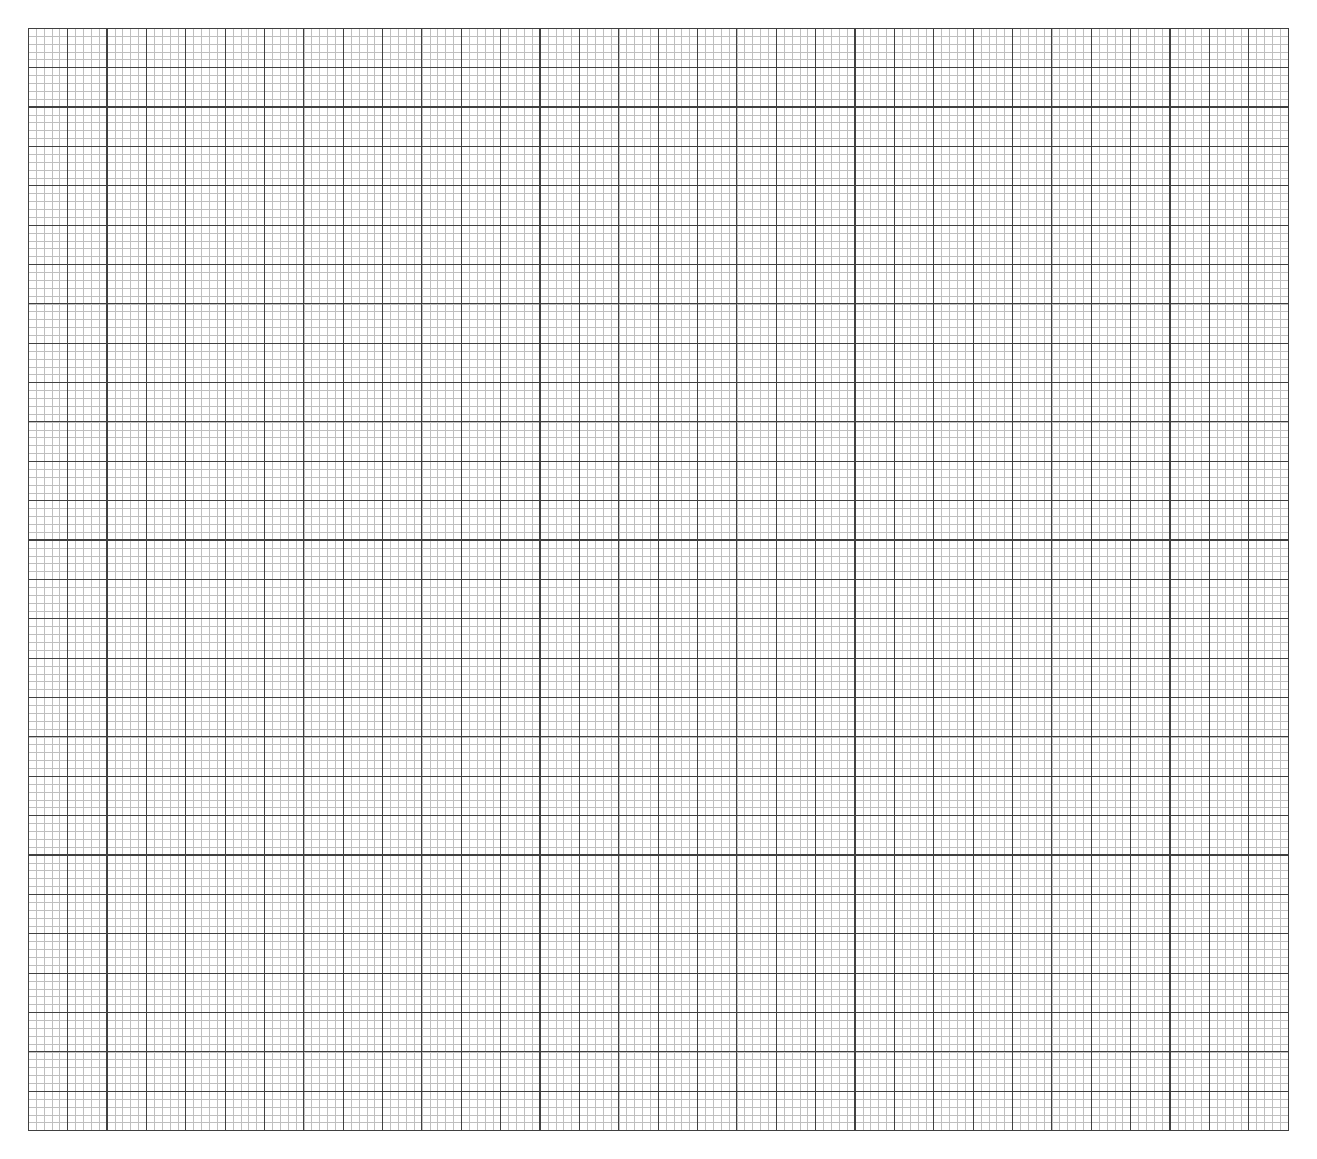
\begin{tikzpicture}[scale=1]
  % Draw the grid (millimeter paper)
  \draw[step=1mm, lightgray, very thin] (0, 0) grid (16, 14); % 1mm steps
  \draw[step=5mm, darkgray, thin] (0, 0) grid (16, 14);    % 5mm steps (darker)
\end{tikzpicture}
    
\end{center}}

\solution{
Achsenbeschriftung und sinnvolle Achsenskalierung (1 P.), jeder richtig eingezeichnete Punkt ($5 \cdot 0,5$ P.), sinnvoll eingezeichnete Ausgleichsgerade (0,5 P.)
$$K_{\mathrm{M}} = 1,74 \mathrm{mmol \cdot L^{-1}} \text{(1 P.)}$$
$$v_{\mathrm{max}} = 284,37 \mathrm{mmol \cdot L^{-1} \cdot s^{-1}} \text{(1 P.)}$$
Insg. 6 P.}{7cm}

\newpage

Die Nullstelle dieser Funktion hat ebenfalls eine Bedeutung.
\enumaufgabe{\operator{Gib} die Nullstelle in Abhängigkeit der Konstanten \operator{an}, welche in \autoref{Michaelis-Menten} auftreten.}
\solution{
\begin{align*}
0 = \frac{K_{\mathrm{M}}}{v_{\mathrm{max}}}\cdot\frac{1}{[\mathrm{S}]_0}+\frac{1}{v_{\mathrm{max}}}\\
\frac{1}{[\mathrm{S}]_0} = -\frac{1}{K_{\mathrm{M}}}\ 
\end{align*}
Insg. 1 P.}{2.8cm}


Zuletzt sollen noch verschiedene Arten der Hemmung betrachtet werden. Es wird zwischen kompetitiver und nicht-kompetitiver Hemmung unterschieden. Bei der kompetitiven Hemmung können Inhibitor und Substrat reversibel an das aktive Zentrum des Enzyms binden, wobei das Enzym ausschließlich aus dem Substrat das Produkt bilden kann. Bei der nicht-kompetitiven Hemmung bindet der Inhibitor an eine andere Stelle des Enzyms und verändert es so, dass der Enzym-Substrat-Komplex nicht zum Produkt reagieren kann, wobei das Binden des Inhibitors keine Auswirkungen auf die Bildung des Enzym-Substrat-Komplexes hat. Für beide Arten der Hemmung ist  in \autoref{Diagramme Hemmung} jeweils ein \textsc{Lineweaver-Burk}-Diagramm gezeichnet.
\begin{figure}[H]
\centering
%\includegraphics[width=0.5\textwidth]{2024/Abbildungen/Kinetik/Ich_habe_Hemmungen.png}
\includegraphics[width=0.6\textwidth]{2024/Abbildungen/Kinetik/Diagramm_1_Süßmaus.png}
\includegraphics[width=0.6\textwidth]{2024/Abbildungen/Kinetik/Diagramm_2_Süßmaus.png}
\caption{Diagramm 1 (oben) und Diagramm 2 (unten) für Teilaufgabe k)}
\label{Diagramme Hemmung}
\end{figure}

\enumaufgabe{\operator{Begründe}, welches Diagramm zu welcher Art der Hemmung gehört.}
\solution{
Diagramm 1: nicht-kompetitive Hemmung, Diagramm 2: kompetitive Hemmung (0,5 P.)\\
Bei der nicht-kompetitiven Hemmung beeinträchtigt der Inhibitor die Enzym-Substrat-Affinität nicht, weshalb $K_{\mathrm{M}}$ gleich bleibt. Aus h) folgt, dass die Nullstelle deshalb an derselben Stelle sein muss, was bei Diagramm 1 der Fall ist (1,5 P.). \\Bei der kompetitiven Hemmung wird die Konzentration des Inhibitors bei großer Substratkonzentration vernachlässigbar klein. Da die Bindung reversibel ist, blockieren die Inhibitor-Moleküle das aktive Zentrum nicht dauerhaft, wodurch die maximale Reaktionsgeschwindigkeit gleich bleibt, was bei Diagramm 2 der Fall ist (1,5 P.)\\
Anmerkung: Es ist nicht zwingend notwendig zu erkennen, dass $K_{\mathrm{M}}$ konstant ist. Alleinige Argumentation über die Maximalgeschwinidgkeit unter Ausschlussverfahren, gibt abenfalls die 1,5P, die für das Erkennen der Konstanz von $K_{\mathrm{M}}$ vorgesehen sind.\\
Insg. 3,5 P.}{5cm}
\enumaufgabe{\operator{Gib an}, wie sich Maximalgeschwindigkeit und sowohl die scheinbare, als auch die echte Enzym-Substrat-Affinität bei den beiden Arten der Hemmung ändern.}
\solution{nicht-kompetitive Hemmung: kleinere Maximalgeschwindigkeit (0,5 P.), gleiche scheinbare und tatsächliche Enzym-Substrat-Affinität (0,5 P.)\\
kompetitive Hemmung: gleiche Maximalgeschwindigkeit (0,5 P.), gleiche tatsächliche Enzym-Substrat-Affinität (0,5 P.), kleinere scheinbare Enzym-Substrat-Affinität (0,5 P.)\\
Insg. 2,5 P.}{3cm}

\solutiontext{$\sum$ 26 P.}{}
\end{document}